\documentclass{standalone}
\usepackage{tikz}
\usetikzlibrary{arrows.meta}
\tikzset{>={Latex[width=3mm,length=3mm]}}
\definecolor{Color1}{RGB}{255,0,0}
\definecolor{Color2}{RGB}{255,128,128}
\definecolor{Color3}{RGB}{255,192,192}
\begin{document}
	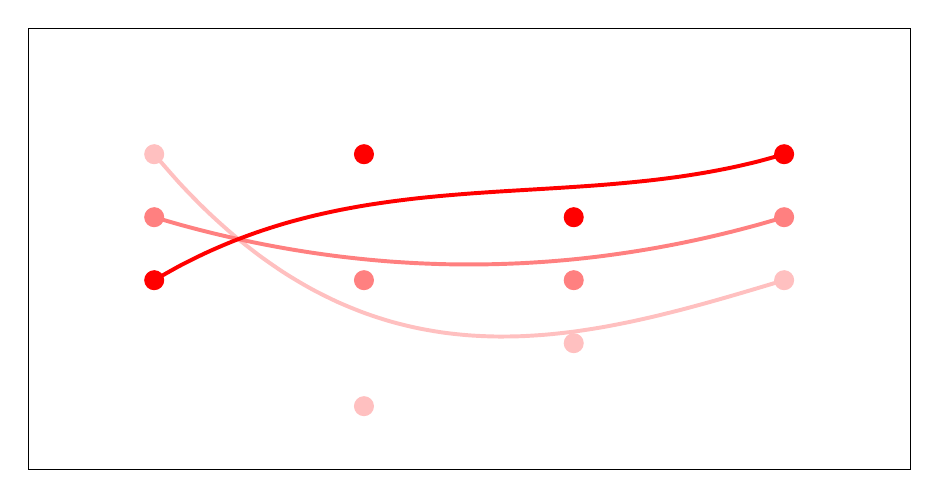
\begin{tikzpicture}[scale=4,x=2cm,y=2cm]
		% border
		\draw (-0.2,0.5) -- (1.2,0.5) -- (1.2,1.2) -- (-0.2,1.2) -- (-0.2,0.5);
		% 1d quadratic bezier curve with control points 0,1,0
		\draw[scale=1,domain=0:1,smooth,variable=\x,Color3,line width=0.5mm] plot ({\x},{1.0*(1-\x)^3 + 0.6*3*(1-\x)^2*\x + 0.7*3*(1-\x)*\x^2 + 0.8*\x^3});	
		\draw[scale=1,domain=0:1,smooth,variable=\x,Color2,line width=0.5mm] plot ({\x},{0.9*(1-\x)^3 + 0.8*3*(1-\x)^2*\x + 0.8*3*(1-\x)*\x^2 + 0.9*\x^3});
		\draw[scale=1,domain=0:1,smooth,variable=\x,Color1,line width=0.5mm] plot ({\x},{0.8*(1-\x)^3 + 1*3*(1-\x)^2*\x + 0.9*3*(1-\x)*\x^2 + 1*\x^3});
		

		% control points
		\draw[red,fill=Color1] (0.0,0.8) circle (0.015);
		\draw[red,fill=Color1] (0.333,1) circle (0.015);
		\draw[red,fill=Color1] (0.666,0.9) circle (0.015);
		\draw[red,fill=Color1] (1,1) circle (0.015);

		%\draw[Color1,->]       (0.0,0.8) -- (0.0,0.9);
		%\draw[Color1,->]       (0.333,1) -- (0.333,0.8);
		%\draw[Color1,->]       (0.666,0.9) -- (0.666,0.8);
		%\draw[Color1,->]       (1.0,1.0) -- (1.0,0.9);

		\draw[Color2,fill=Color2] (0.0,0.9) circle (0.015);
		\draw[Color2,fill=Color2] (0.333,0.8) circle (0.015);
		\draw[Color2,fill=Color2] (0.666,0.8) circle (0.015);
		\draw[Color2,fill=Color2] (1,0.9) circle (0.015);

		%\draw[Color2,->]       (0.0,0.9) -- (0.0,1.0);
		%\draw[Color2,->]       (0.333,0.8) -- (0.333,0.6);
		%\draw[Color2,->]       (0.666,0.8) -- (0.666,0.7);
		%\draw[Color2,->]       (1.0,0.9) -- (1.0,0.8);				

		\draw[Color3,fill=Color3] (0.0,1.0) circle (0.015);
		\draw[Color3,fill=Color3] (0.333,0.6) circle (0.015);
		\draw[Color3,fill=Color3] (0.666,0.7) circle (0.015);
		\draw[Color3,fill=Color3] (1,0.8) circle (0.015);			
	\end{tikzpicture}
\end{document}

% A*s^3      : 0.8 -> 0.9  -> 1.0
% B*3*s^2*t  : 1   -> 0.8 - > 0.6
% C*3*s*t^2  : 0.9 -> 0.8  -> 0.7
% D*t^3      : 1   -> 0.9  -> 0.8